\documentclass[a4paper,10pt, oneside]{book}


%--- Useages
\usepackage[utf8]{inputenc}
\usepackage[english]{babel}
\usepackage{textcomp}

% --- color text
\usepackage{color}

%---- Format correctly ----
\usepackage[left=2cm, right=2cm, bottom=3cm, top=2cm]{geometry}

%---- Preamble -----
\title{NP Zusammenfassung}
\author{Lukas Schaller}
\date{\today}

%--- Mathematik -----
\usepackage{amsmath, amssymb, amstext}
\usepackage{dsfont}
\usepackage{ stmaryrd } % für die Klammern

%--- Pictures ----
\usepackage{graphicx}
\graphicspath{ {./images/} }

\begin{document}
\maketitle
\tableofcontents

\chapter{A1}
\section{Aktionen}
\paragraph{Actionen}
Seien \textit{Kom} eine Menge von Kommunikationsaktionen und \textit{Int} eine davon disjunkte Menge von internen Aktionen. Dann ist
\begin{equation*}
 Act = Kom \cup Int
\end{equation*}
die Menge aller Aktionen. Dabei gelten folgende Konventionen:

$ \alpha, \beta, \gamma, ... \in Act$ \quad\quad
$ a,b,c,... \in Int$ \quad\quad
$ [a],[b],[c],... \in Kom$ \quad\quad

\paragraph{Transitionssystem (LTS)}
Ein beschritetes Transitionssystem TS ist ein Tripel ($S, \longrightarrow, s_0$), wobei
\begin{itemize}
 \item $S$ die Zustandsmenge
 \item $\longrightarrow \subseteq S \times Act \times S$ die Transitionsrelation,
 \item $s_0 \in S$ der initiale Zustand ist
\end{itemize}


\paragraph{Nachfolger}
Sei ein LTS $TS$ = ($S$, $\rightarrow$, $s_0$) gegeben. Sei $s \in S$, $C \subseteq S$, $ \alpha \in Act$, und $A \subseteq Act$.

\begin{flushleft}
 $Post(s,\alpha) = \{s' \in S | s \xrightarrow{\alpha} s'\}$, 
\end{flushleft}

\begin{flushright}
 $Post(s,A) = \bigcup\limits_{\alpha \in A} Post(s,\alpha)$
\end{flushright}


\begin{flushleft}
 $Post(C,\alpha) = \bigcup\limits_{s \in C} Post(s,\alpha)$,
\end{flushleft}

\begin{flushright}
 $Post(C,A) = \bigcup\limits_{\alpha \in A} Post(C,\alpha)$
\end{flushright}

Aktionen die in Zusand s als nächstes möglich sind:
\begin{equation*}
 Act(s) = \{\alpha \in Act \; | \; \exists s': s \xrightarrow{\alpha} s'\}
\end{equation*}
Aktionen, die in Zustand s als nächstes beobachtet werden können:
\begin{equation*}
 Kom(s) = \{\alpha \in Kom \; | \; \exists s': s \xrightarrow{\alpha} s'\}
\end{equation*}


\paragraph{Erreichbarkeit}
$Reach(s)$ ist die Menge aller von s erreichbaren Zustände in $TS$
\begin{equation*}
 Reach(s) = \bigcup\limits_{n \in \mathds{N}} Post^n(s)
\end{equation*}
wobei $Post^0(s) = {s}$ und $Post^{n+1}(s) = Post(Post^n(s), Act)$

\section{Trainingsblatt}
\subsubsection{Vorgänger}
$Pre(s,\alpha) = \{s' \in S | s' \xrightarrow{\alpha} s\}$, 
\hfill
$Pre(s,A) = \bigcup\limits_{\alpha \in A} Pre(s,\alpha)$

\begin{flushleft}
$Pre(C,\alpha) = \bigcup\limits_{s \in C} Pre(s,\alpha)$,
\hfill
$Pre(C,A) = \bigcup\limits_{\alpha \in A} Pre(C,\alpha)$
\end{flushleft}

\paragraph{terminaler Zustand}
Ein terminaler Zustand ist ein Zustand ohne Nachfolger. Ein Zustand ist genau dann terminal wenn $Act(s) = \emptyset$.

\paragraph{Alphabet des LTS}
Alphabet eines LTS $TS = \bigcup\limits_{s \in Reach(TS)} Kom(s)$

\section{Nichtdeterminismus}
\paragraph{Nichtdeterminismus}
Sei $Post(s) = Post(s, Act)$ und es sei ein LTS $TS = (S, \rightarrow, s_0) $ gegeben. $TS$ ist deterministisch genau dann wenn für alle $s \in S$,

\begin{center}
$ |Post(s)| \leq 1 $ und $|Act(s)| \leq 1$
\end{center}

Andernfalls heißt das $TS$ nichtdeterministisch!

\paragraph{Interner und Externer Nichtdeterminismus}
\begin{flushleft}
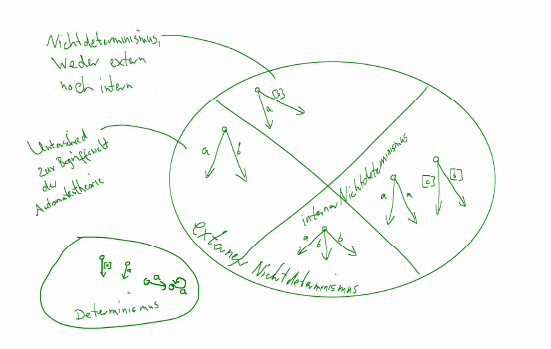
\includegraphics[scale=1]{chart_nichtdeterministisch} 
\end{flushleft}

\subsection{Annahmen nebenläufiger Prozesse}
\begin{itemize}
 \item Zeit wird nur bezüglich relativen Geschwindigkeit der Prozesse untereinander betrachtet, nicht absolut.\\
 Jeder Prozess kann gerade beliebig schnell oder langsam voranschreiten.
 \item Aktionen sind unteilbar und zeitlos.
 \item Nebenläufige Prozesse agieren komplett voneinander unabhängig und unbeeinflusst, es sei denn, sie kommunizieren explizit miteinander.
\end{itemize}

\section{Labled Transitionsystem}
\begin{flushleft}
 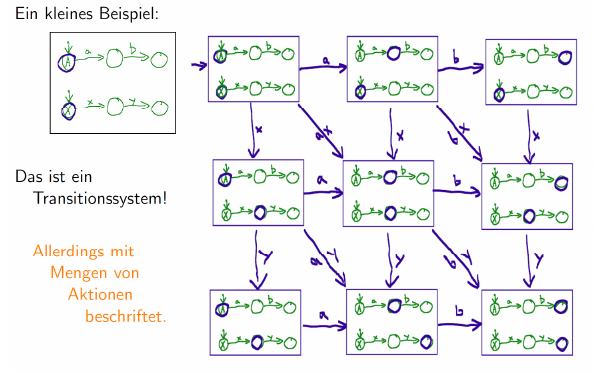
\includegraphics{lts.png}
 \textbf{Hinweis:} Die diagonalen Kanten können wegen der Zeitlosigkeit der Aktionen auch weggelassen werden.
\end{flushleft}


\chapter{B1 - CSS}
\section{$CSS_0$}
\subsection{Syntax}
Gegeben sei die Menge aller Aktionen $Act$. Dann ist die Menge aller Ausdrücke in $CSS_0$ gegeben durch:
\begin{equation*}
 P \; ::= \; 0 \; | \; P \: + \: P \; | \; \alpha.P
\end{equation*}
wobei $\alpha \in Act$.

\subsubsection{Klammersparregeln}
\begin{itemize}
 \item '+' klammert links: $ P + Q + R \rightsquigarrow (P + Q) + R$
 \item '.' klammert rechts: $ \alpha.\beta.P \rightsquigarrow \alpha.(\beta.P)$
 \item Punkt vor Strich: $ \alpha.P + Q \rightsquigarrow (\alpha.P) + Q $
\end{itemize}

\subsection{Semantik}
Die Semantik einer Sprache beschreibt, welches mathematische Objekt mit einem Ausdruck der Sprache assoziiert werden soll. Die Semantik des Ausdrucks $P$ aus $CCS_0$ ist ein LTS $\llbracket P \rrbracket = (S, \rightarrow, s_0)$.
\begin{itemize}
 \item Zustandsmenge S ist die Menge aller $CCS_0$-Ausdrücke
 \item $s_0 = P$
 \item $\longrightarrow$ ist eine Teilmenge von $(CSS_0 \times Act \times CCS_0)$
\end{itemize}

\subsubsection{Inferenzregeln}
\begin{flushleft}
Hinweis: $CCS_0$ beinhaltet noch nicht die Inferenzregeln $rec$
\end{flushleft}
\begin{center}
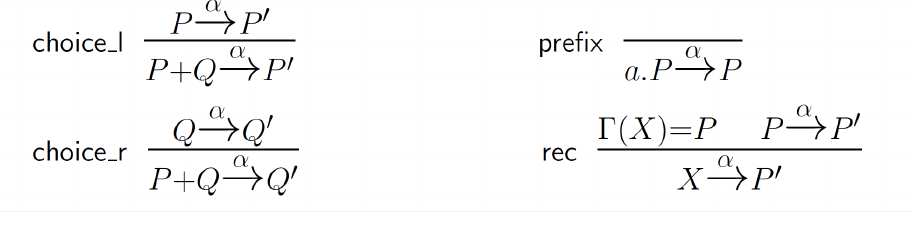
\includegraphics[scale=0.4]{inferenzregeln}
\end{center}

\subsubsection{Isomorphie}
Zwei Transitionssysteme $TS = (S,\rightarrow, s_0)$ und $TS' = (S', \rightarrow', s'_0)$ sind isomorph $(TS \sim_{iso} TS')$, wenn es eine Bijektion $f$ gibt mit $f: Reach(TS) \rightarrow Reach(TS)$, so dass $f(s_0) = s'_0$ und für alle $s_1, s_2 \in Reach(TS)$ und alle $\alpha \in Act$ gilt: $s_1 \xrightarrow{\alpha} s_2 $ genau dann wenn $f(s_1) \xrightarrow{\alpha}' f(s_2) $.\\
\begin{flushleft}
\underline{Intuition}: Zwei LTS sind isomorph solange sie sich ausschließlich im Namen der Zustände unterscheiden. Die Transitionen müssen gleich bleiben!
\end{flushleft}

\paragraph{Satz}
Für jedes endliche azyklische LTS $TS$ gibt es einen Ausdruck $P \in CCS_0$, so dass $TS \sim_{iso} \llbracket P \rrbracket$.

\section{$CCS_0^{\omega}$}
\subsection{Semantik}
Gegeben sei die Menge aller Aktionen $Act$ und eine Menge von Rekursionsvariablen $Var$. Dann ist die Menge der Ausdrücke in $CCS_0^{\omega}$ wie folgt:\\
\begin{center}
$ P \: ::= \: o \: | \: X \: | \: P \: + \: P \: | \: \alpha.P $ , wobei $\alpha \in Act$ und $X \in Var$ 
\end{center}

\subsubsection{Beispiele}
$ X := a.b.Y $\\
$ Y := b.Z + a.Y $\\
$ Z := a.Y $
\begin{flushleft}
Eine Menge solcher Gleichungen definiert offensichtlich eine partielle Funktion: $\Gamma \in Var \rightharpoonup CCS_0^{\omega}$. In diesem Beispiel ergibt sich demnach: $\Gamma = \{(X,a.b.Y),(Y,b.Z + a.Y),(Z,a.Y)\}$

\bigbreak

Es soll gelten:
\begin{itemize}
 \item $(\alpha.P,\alpha,P) \in \rightarrow ;$
 \item $ (P + Q, \alpha, P') \in \rightarrow$ , wann immer $(P,\alpha,P') \in \rightarrow$ ;
 \item $ (P + Q,\alpha, Q') \in \rightarrow$ , wann immer $(Q,\alpha,Q') \in \rightarrow$ ;
 \item $(X,\alpha,P') \; \in \; \rightarrow$, wann immer $\Gamma(x) = P$ und $ (P, \alpha, P') \in \rightarrow$ ;
 \item nichts sonst ist Element von $\rightarrow_{\Gamma}$
\end{itemize}
 
\end{flushleft}

\subsection{Geschützte Ausdrücke}
Eine Variable $X$ ist geschützt in einem Ausdruck $P$, wenn jedes Auftreten von $X$ in $P$ in einem Teilausdruck von $P$ der Form $\alpha.Q$ enthalten ist. Andernfalls heißt $X$ ungeschützt.\\
Ein Ausdruck $P$ heißt geschützt, wenn alle darin vorgekommenden Variablen in $P$ geschützt sind. Andernfalls heißt $P$ ungeschützt.

\subsubsection{Beispiele}

 ungeschützte Ausdrücke: $X$, $\tau.X + Y$, $(a.X) + X$
\hfill
geschützte Ausdrücke: $\alpha.X$, $\tau.(X + Y)$, $\alpha.(X + b.X)$

\section{Sequentielles $CSS_0^{\omega}$}
Für eine Bindung $\Gamma: Var \rightharpoonup CCS_0^{\omega}$ sei $ \rightarrow_{\Gamma} \subseteq CCS_0^{\Gamma} \times Act \times CCS_0^{\Gamma}$ die kleinste Relation $\longrightarrow$, die den Inferenzregeln genügen.

\subsection{Semantik}
Sei $LTS_0^{\omega} = \{(CCS_0^{\omega}, T, s) | T \subseteq CCS_0^{\omega} \times Act \times CCS_0^{\omega}, s \in CCS_0^{\omega}\}$. Die Semantik von $CCS_0^{\omega}$ ist eine (kaskadierte) Funktion:\\
\begin{center}
 $\llbracket\_\rrbracket \; : \; (Var \rightharpoonup CCS_0^{\omega}) \; \rightarrow \; CCS_0^{\omega} \; \rightarrow \;  LTS_0^{\omega}$\\
 $\llbracket\_\rrbracket \; \Gamma \; P \; = \; (CCS_0^{\omega}, \rightarrow_{\Gamma}, P)$
\end{center}
Wir schreiben $\llbracket P \rrbracket_{\Gamma}$ für $\llbracket \_ \rrbracket \: \Gamma \: P$, oder auch nur $\llbracket P \rrbracket$, sofern $\Gamma$ aus dem Kontext heraus klar ist.

\paragraph{Satz}
Für jedes endliche LTS $TS$ gibt es einen Ausdruck $P \in CCS_0^{\omega}$ und eine endliche Bindung $\Gamma$, sodass $TS \sim_{iso} \llbracket P \rrbracket_{\Gamma}$

\subsubsection{Zusätzliche Inferenzregeln}
TODO: Hier Bild von par\_l und par\_r einfügen

\subsection{Synchronisation}
Synchronisation bietet die Grundlage um unterschiedliche Prozesse auf Aktionen reagieren zu lassen. So kann zum Beispiel die 'light'-Aktion des Feuerzeug-Prozesses in einem Prozess eines Chinaböllers die passive Aktion 'light' hervorrufen.
In CSS machen wir dazu die Kommunikationsaktionen entweder 'aktiv' oder 'passiv'. Statt einer beliebigen Menge $Kom$ von Markierungen verwenden wir eine Menge, die mehr Struktur aufweist:\\
$Kom = A^! \bigcup A^?$. Aktionen mit '!' als Output-Aktionen (aktiv) und Aktionen mit '?' als Input-Aktionen interpretiert werden.


\paragraph{Komplementarität}
Input- und Output-Aktionen treten als Paare auf. Das Komplement von $a \in A^! \bigcup A^?$ ist $\bar{a}$. Auch für interne Aktionen $\tau$ gilt $\tau = \bar{\tau}$. Das doppelte Komplement hebt die Wirkung auf: $\alpha \in Act: \bar{\bar{a}} = \alpha$

\paragraph{Hinweis} Interne Aktionen können NICHT synchronisieren.

\subsubsection{Zusätliche Inferenzregel}
\begin{center}
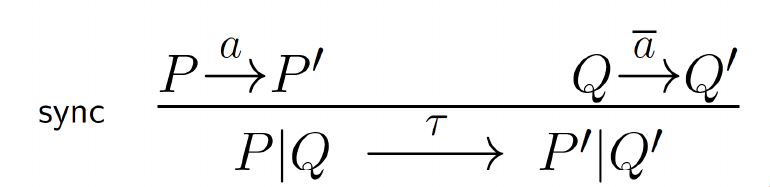
\includegraphics[scale=0.3]{sync_regel}
\end{center}

\subsection{Restriktions-Operator}
Der Restriktions-Operator '\' unterbindet bestimmte (Paare von) Aktionen eines Prozesses. Intuitiv gesprochen erzwingt er eine Synchronisation.\\
\textbf{P\textbackslash H} ist ein zweistelliger Operator, mit \textbf{P} als CCS-Ausdruck und \textbf{H} als menge von Kommunikationsaktionen, die unterbunden werden sollen.

\paragraph{Inferenzregel}
\begin{center}
 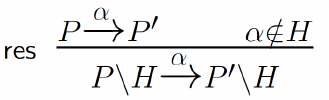
\includegraphics[scale=0.6]{res_regel}
\end{center}

Annahmen über zulässige Menge H:
\begin{itemize}
 \item Die interne Aktion kann nicht unterbunden werden: $\tau \notin H$
 \item Aktionen treten in H paarweise auf: $a \in H \Longleftrightarrow \bar{a} \in H$
\end{itemize}

\section{Volle CCS-Power}
\subsection{Syntax}
Gegeben sei die Menge aller Kommunikationsaktionen $Kom = A^! \bigcup A^?$, $Act = Kom \bigcup \{ \tau \}$ und eine Menge von Rekursionsvariablen $Var$. Dann ist die Menge aller Ausdrücke in $CCS$ wie folgt gegeben: \\
\begin{equation*}
 P \; ::= \; 0 \; | \; X \; | \; P \: + \: P \; | \; \alpha.P \; | \; P|P \; | \; P\backslash H
\end{equation*}
wobei $\alpha \in Act, X \in Var$ und $H \subseteq Kom$.

\subsection{Semantik}
Die Semantik der Ausdrücke con CCS ist gegeben durch:\\
\begin{center}
 $\llbracket\_\rrbracket \; : \; (Var \rightharpoonup CCS) \; \rightarrow \; CCS \; \rightarrow \;  LTS^{CCS}$\\
 $\llbracket\_\rrbracket \; \Gamma \; P \; = \; (CCS, \rightarrow_{\Gamma}, P)$
\end{center}
wobei $LTS^{CCS} = \{(CCS, T, s) | T \subseteq CCS \times Act \times CCS, s \in CCS\}$ uns $\rightarrow_{\tau}$ die kleinste Relation $\rightarrow$ ist, die den folgenden Regeln genügt.

\paragraph{Inferenzregeln}
\begin{center}
 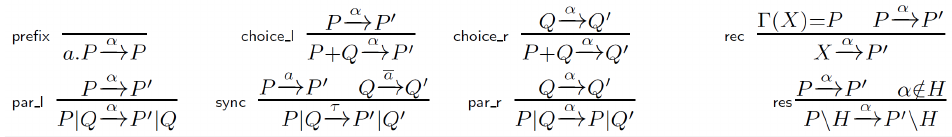
\includegraphics[scale=0.6]{inferenz_ges}
\end{center}

\subsection{Regulärer Ausdruck}
Ein CCS-Asdruck wird regulär genannt, wenn er durch folgende Grammatik gebildet werden kann:
\begin{center}
 $ P \ ::= \  0 \ | \ X \ | \ P+P \ | \ \alpha.P \ | \ R$\\
 $ R \ ::= \ 0 \ | \ R+R \ |\  \alpha.R  \ | \ R|R \ | \ R\backslash H $
\end{center}

\paragraph{Satz}
Sofern $\Gamma$ eine endliche Bindung ist bei der alle rechten Seiten regulär sind, ist $Reach(\llbracket P \llbracket_{\Gamma})$ für jedes $P \subset CCS$ endlich.

\chapter{C1}
Dieses Kapitel befasst sich mit der beobachtbarem Verhalten von Prozessen. Die Kommunikationsaktionen und die Spuren (mögliche Aktionsfolgen) lassen sich beobachten. Die internen Aktionen und die durchlaufenden Zustände lassen sich offensichtlich nicht beobachten!

\subsubsection*{Definition: Spuren}
Sei $TS = (S,\rightarrow,s_0)$ ein LTS. Dann definieren wir die Funktion LTS $\rightarrow 2^{Act^*}$ als 
\begin{equation*}
Traces(TS) := \{\alpha_1\alpha_2...\alpha_n \in Act^* | n \geq 0 \exists s_1, ... , s_n : \forall 0 < i \leq n : s_{i-1} \xrightarrow{\alpha_i} s_i\}
\end{equation*}
als die Menge der endlichen Spuren von $TS$. Wir schreiben $s_0 \rightsquigarrow^{\varrho} s'$

\subsubsection*{Definition: Kongruenzrelation}
Eine Äquivalenzrelation $\approx$ auf $CCS$ ist eine Kongruenzrelation, wenn für alle CCS-Ausdrücke $P, Q$ und alle Kontexte $C[.]$, $P \approx Q$ impliziert, dass $C[P] \approx C[Q]$ gilt.

\begin{center}
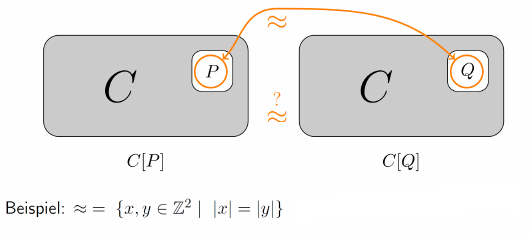
\includegraphics[scale=0.6]{kongruenzrelation}
\end{center}

\underline{Algebraische Gesetze}:\\
\begin{center}
\begin{tabular}{ c r }
 $P + Q \sim_{tr} Q + P$ & Kommutativität von +\\
 $(P + Q) + R \sim_{tr} P + (Q + R)$ & Assozitivität von +\\
 $P + 0 \sim_{tr} P$ & 0 als neutrales Element von +\\
\end{tabular}
\end{center}

\subsubsection{Spuräquivalenz}
Sei $\Gamma$ : $Var \rightharpoonup CCS, P, Q, R \in CCS$ und $H \subseteq Kom$ sowie $\alpha \in Act$. Wenn $P \sim_{tr} Q$, dann auch:
\begin{center}
\begin{tabular}{c c c}
$P + R \sim_{tr} Q + R$ & \quad\quad $R + P \sim_{tr} R + Q$ & \quad\quad $P | Q \sim_{tr} Q | R$\\
$R | P \sim_{tr} R | Q$ & $\alpha.P \sim_{tr} \alpha.Q$ & $P\backslash H \sim_{tr} Q\backslash H$
\end{tabular}
\end{center}

\section{Verklemmung}
Ein Zustand $s$ ist terminal, falls $Post(s, Act) = \emptyset$. Wir schreiben dann $s \nrightarrow$. Falls $P$ in $\llbracket P \rrbracket_{\Gamma}$ terminal ist, nennen wir $P$ einen verklemmten Prozess.

\paragraph{Terminierende Spuren}
Die \textcolor{blue}{terminierenden Spuren} eines Prozesses $P$ sind alle Spuren, die einem terminalen Zusand enden.

 $TTraces(P) = TTraces(\llbracket P \rrbracket_{\Gamma})$\\
 $TTraces(\llbracket P \rrbracket) := \{\varrho \in Traces(\llbracket P \rrbracket_{\Gamma}) | \exists P':P \rightsquigarrow^{\varrho} P' \wedge P' \nrightarrow\}$
\\

Beispiele:
\begin{itemize}
 \item Traces(a!.b!.0 + a!.0) $=$ \textbraceleft $\epsilon$,a!,a! b!\textbraceright
 \item Traces(a!.b!.0) $=$ \textbraceleft $\epsilon$,a!,a! b!\textbraceright
 \item TTraces(a!.b!.0 + a!.0) = \textbraceleft a!,a! b!\textbraceright
 \item TTraces(a!.b!.0) = \textbraceleft a! b!\textbraceright
\end{itemize}

\section{Gleichheit}
Die 'Super'-Gleichheit...
\begin{itemize}
 \item ist eine Äquivalenzrelation
 \item ist eine Kongruenzrelation
 \item erhält Spuren
 \item ist verklemmungssensitiv (erhält terminierende Spuren)
 \item ist grob genug (gröber als $\sim_{iso}$)
\end{itemize}

\section{(Starke) Bisimilarität}
Zwei Prozesse sind äquivalent, wenn sie zustandsweise gleich sind. 'Gleiche' Zustände erlauben Tranisitionen mit den gleichen Aktionen, die wieder in 'gleichen' Zuständen landen.\\
\\
Eine Relation $R \subseteq S \times S$ über den Zuständen eines LTS $TS = (S,\rightarrow,s_0)$ ist eine (starke) Bisimulation, wenn für alle $P,Q \in S$ mit $(P,Q) \in R$ und für alle $\alpha \in Act$ gilt:

\begin{itemize}
 \item Für jedes $P' \in S$ mit $P \xrightarrow{\alpha} P'$ gilt: Es gibt ein $Q' \in S$ mit $Q \xrightarrow{\alpha} Q'$ und $(P',Q') \in R$.
 \item Für jedes $Q' \in S$ mit $Q \xrightarrow{\alpha} Q'$ gilt: Es gibt ein $P' \in S$ mit $P' \xrightarrow{\alpha} P'$ und $(P', Q') \in R$.
\end{itemize}
Zwei Zustände heißen bisimilar wenn es eine Bisimulation $R$ gibt mit $(P,Q) \in R$.

\begin{center}
$ \sim $ \quad := \quad $\bigcup_{R ist eine Bisimulation} R$\\
$ (P,Q) \: \in \: \sim \quad \Leftrightarrow \quad \exists$ Bisimulation $R : (P,Q) \in R \Leftrightarrow P$ und $Q$ sind bisimilar
\end{center}
$\sim$ ist die Relation aller zueinander bisimilaren Zustände. Sie heißt \textbf{Bisimilarität}. Gleichzeitig ist $\sim$ eine Bisimulation, und zwar die größtmögliche.

\subsection*{Algebra der Bisimilarität}
Zwei Prozesse $P,Q \in CCS_0$ sind genau dann bisimilar $(P \sim Q)$, wenn sie sich durch Anwenden der folgenden Axiome syntaktisch ineinander umgeformt werden können:
\begin{itemize}
 \item $P + Q \sim Q + P$
 \item $(P + Q) + R \sim P + (Q + R)$
 \item $(P + 0 \sim P$
 \item $P + P \sim P$
\end{itemize}

\section{Minimale Repräsentanten eines LTS}
Hier wird das \textit{kleinste} LTS, das bisimilar zu dem gegebenen LTS ist, gesucht. Der gefundene Repräsentant ist bis auf Isomorphie eindeutig!

\subsubsection*{Algorithmus}
\begin{enumerate}
 \item Gehe davon aus, dass alle Zustände gleich (im Sinne von Bisimilarität) sind
 \item Suche solange Argumente, warum Zustände noch verschieden sind, bis die Zustände in ihre Äquivalenzklassen getrennt sind
 \item Fasse Zustände einer Äquivalenzklasse Zusammenfassung
 \item Lösche doppelte Transitionen
\end{enumerate}

\chapter*{Kapitel D}
\section{Definitionen}
\subsubsection{Spur : $P \overset{\sigma}{\rightsquigarrow} Q$}
Für $\sigma = \alpha_1 ... \alpha_n \in Act*$ schreiben wir $P \overset{\sigma}{\rightsquigarrow} Q$, falls $\sigma = \varepsilon$ und $P = Q$ oder es einen Zustand $s_0, ... , s_n$ gibt, mit $s_{i-1} \xrightarrow{\alpha_i} s_i$ für i = 1,...,n und $P = s_0$ und $Q = s_n$

\subsubsection*{Schwache Bisimulation $s \approx t$}
\begin{itemize}
 \item wenn $s \overset{\alpha}{\Rightarrow} s'$, dann gibt es eine Transition $t \overset{\alpha}{\Rightarrow} t'$, so dass s' $R$ t'
 \item wenn $t \overset{\alpha}{\Rightarrow} t'$, dann gibt es eine Transition $s \overset{\alpha}{\Rightarrow} s'$, so dass s' $R$ t'
\end{itemize}

\subsubsection*{Auswahl-Kongruenz: $\approx^+$}
Zwei Ausdrücke $P,Q \in CCS_0$ heißen genau dann Auswahl-Kongruent, gschrieben $P \approx^+ Q$, wenn für alle $R \in CCS_0$ gilt:
\begin{center}
 $P + R \approx Q + R$
\end{center}

\subsubsection*{Beobachtungskongruenz: $\overset{\sim}{=}$}
\begin{itemize}
 \item wenn $P \xrightarrow{\alpha} P'$, dann $\exists (n,m) \in \mathds{N}^2: Q \overset{\tau^n \alpha \tau^m}{\rightsquigarrow} Q' \wedge P' \approx Q'$
 \item wenn $Q \xrightarrow{\alpha} Q'$, dann $\exists (n,m) \in \mathds{N}^2: P \overset{\tau^n \alpha \tau^m}{\rightsquigarrow} P' \wedge P' \approx Q'$
\end{itemize}

Es gilt außerdem: $P \overset{\sim}{=} Q \: \Leftrightarrow \: P =^+ Q$

\subsubsection*{Schwache Transition: $\Longrightarrow$}
Sei ein LTS $TS = (S,\rightarrow,s_0)$ gegeben. Wir definieren die Transitionsrelation $\Longrightarrow \subset S \times Act \times S$ wie folgt:
\begin{itemize}
 \item $s \overset{\tau}{\Longrightarrow} s': \Leftrightarrow \exists n \geq 0: s \overset{\tau^n}{\rightsquigarrow} s'$
 \item $s \overset{a}{\Longrightarrow} s': \Leftrightarrow \exists s'',s''' \in S: s \overset{\tau}{\Rightarrow} s'' \xrightarrow{a} s''' \overset{\tau}{\Rightarrow} s'$
\end{itemize}
mit $a \in Kom$. Beachte dass auch $s'' = s$ und $s''' = s'$ möglich ist.


\subsubsection*{Weak Traces: $\sim_{wtr}$}
$WTraces(P) = \{a_1 a_2 ... a_n | \tau^* a_1 \tau^* a_2 \tau^* ... \tau^* a_n \tau^* \in Traces(P)\}$


\subsubsection{Schwache Spuräquivalenz: $P \sim_{wtr} Q$}
P und Q sind schwach Spuräquivalent $P \sim_{wtr} Q$, genau dann wenn $WTraces(\llbracket P \rrbracket_{\Gamma}) = WTraces(\llbracket Q \rrbracket_{\Gamma})$ gilt 

\section{$CCS_{vp}$}
\subsection*{Syntax}
Die Menge aller Ausdrücke in $CCS_{vp}^{\mathds{Z}}$ ist durch die folgende Grammatik gegeben:
\begin{center}
 $P ::= 0 \quad | \quad X[u_1,...,u_n] \quad | \quad P + P \quad | \quad \alpha.P \quad | \quad P | P \quad | \quad P\backslash H \quad | \quad when(b) P$,
\end{center}
wobei
\begin{center}
 $\alpha ::= \quad \tau \quad | \quad a! \quad | \quad a? \quad | \quad a!v \quad | \quad a?v \quad | \quad a!x \quad | \quad a?x$
\end{center}
und $a \in \mathds{K}$, $X \in Var$, $H \subseteq Kom$, $v \in \mathds{V}$, $x \in D$ sowie $r_i \in D \cup \mathds{V} \cup \mathds{K}$.

\subsection*{Semantik}
Die Regeln aus CCS werden um folgende Regeln erweitert bzw prefix wird abgeändert:
\begin{center}
 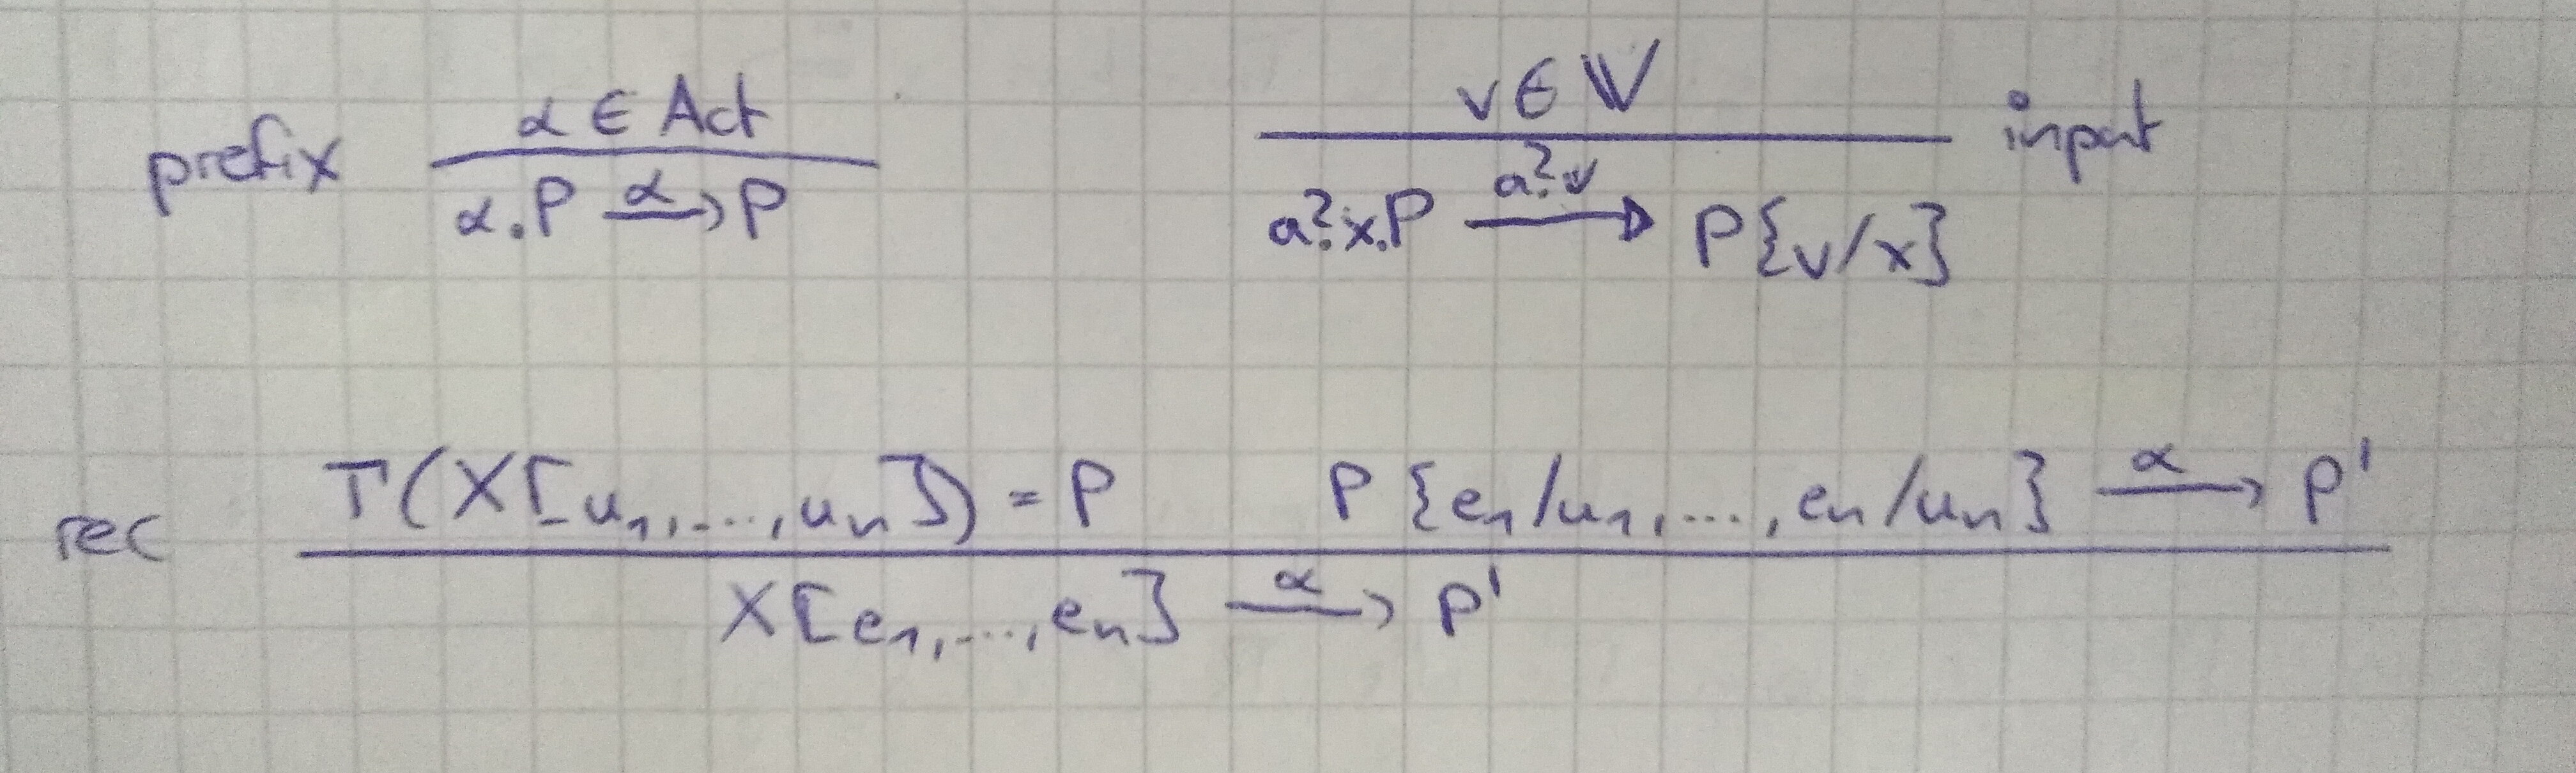
\includegraphics[scale=0.08]{CCSvp}
\end{center}


\section{$CCS_{vp}^{\mathds{Z}}$}
\subsection*{Syntax}
Die Menge aller Ausdrücke in $CCS_{vp}^{\mathds{Z}}$ ist durch die folgende Grammatik gegeben:
\begin{center}
 $P ::= 0 \quad | \quad X[u_1,...,u_n] \quad | \quad P + P \quad | \quad \alpha.P \quad | \quad P | P \quad | \quad P\backslash H \quad | \quad when(b) P$,
\end{center}
wobei
\begin{center}
 $\alpha ::= \quad \tau \quad | \quad a! \quad | \quad a? \quad | \quad a!e \quad | \quad a?x$
\end{center}
und $X \in Var$, $H \subseteq Kom$, $a \in \mathds{K} \cup D$, $e \in AExp, b \in BExp$, $x \in D$ sowie $u_i \in AExp \cup \mathds{K}$.

\subsection*{Semantik von $CCS_{vp}^{\mathds{Z}}$}
\begin{center}
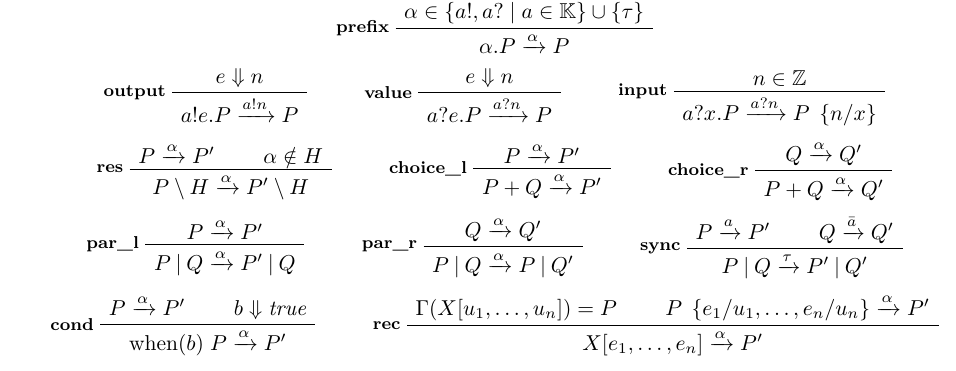
\includegraphics[scale=0.7]{CCSvpz}
\end{center}

\subsection{Ersetzung formell}
\begin{tabular}{l c l}
 $0\{v/x\}$ & = & 0\\
 $(P + Q) \{v/x\}$ & = & $P\{v/x\} + Q\{v/x\}$\\
 $(P | Q) \{v/x\}$ & = & $P\{v/x\} \; | \; Q\{v/x\}$\\
 $(\alpha.P) \{v/x\}$ & = & $P\{v/x\} \backslash \{\alpha \{v/x\} \; | \; \alpha \in H\}$\\
 $a?$ oder $a! \{v/x\}$ & = & $a?$ oder $a!$, falls $ a \neq x$\\
 & & $v?$ oder $v!$, falls $a = x$\\
 $\tau \{v/x\}$ & = & $\tau$\\
 $(a?y.P) \{v/x\}$ & = & $a? \{x/v\}y.P\{v/x\}$, falls $x \neq y$\\ 
 & & $a? \{x/v\}y.P$, falls $x = y$\\ 
 $(a!y.P) \{v/x\}$ & = & $a! \{x/v\}y.P\{v/x\}$, falls $x \neq y$\\ 
 & & $a! \{x/v\}y.P$, falls $x = y$\\ 
 $X[y_1,...] \{x/v\}$ & = & $X[y_1,...]$, falls $x \neq y$\\
 & & $X[v,...]$, sonst
\end{tabular}

\subsubsection*{Variable vs Ausdruck:}
\begin{center}
 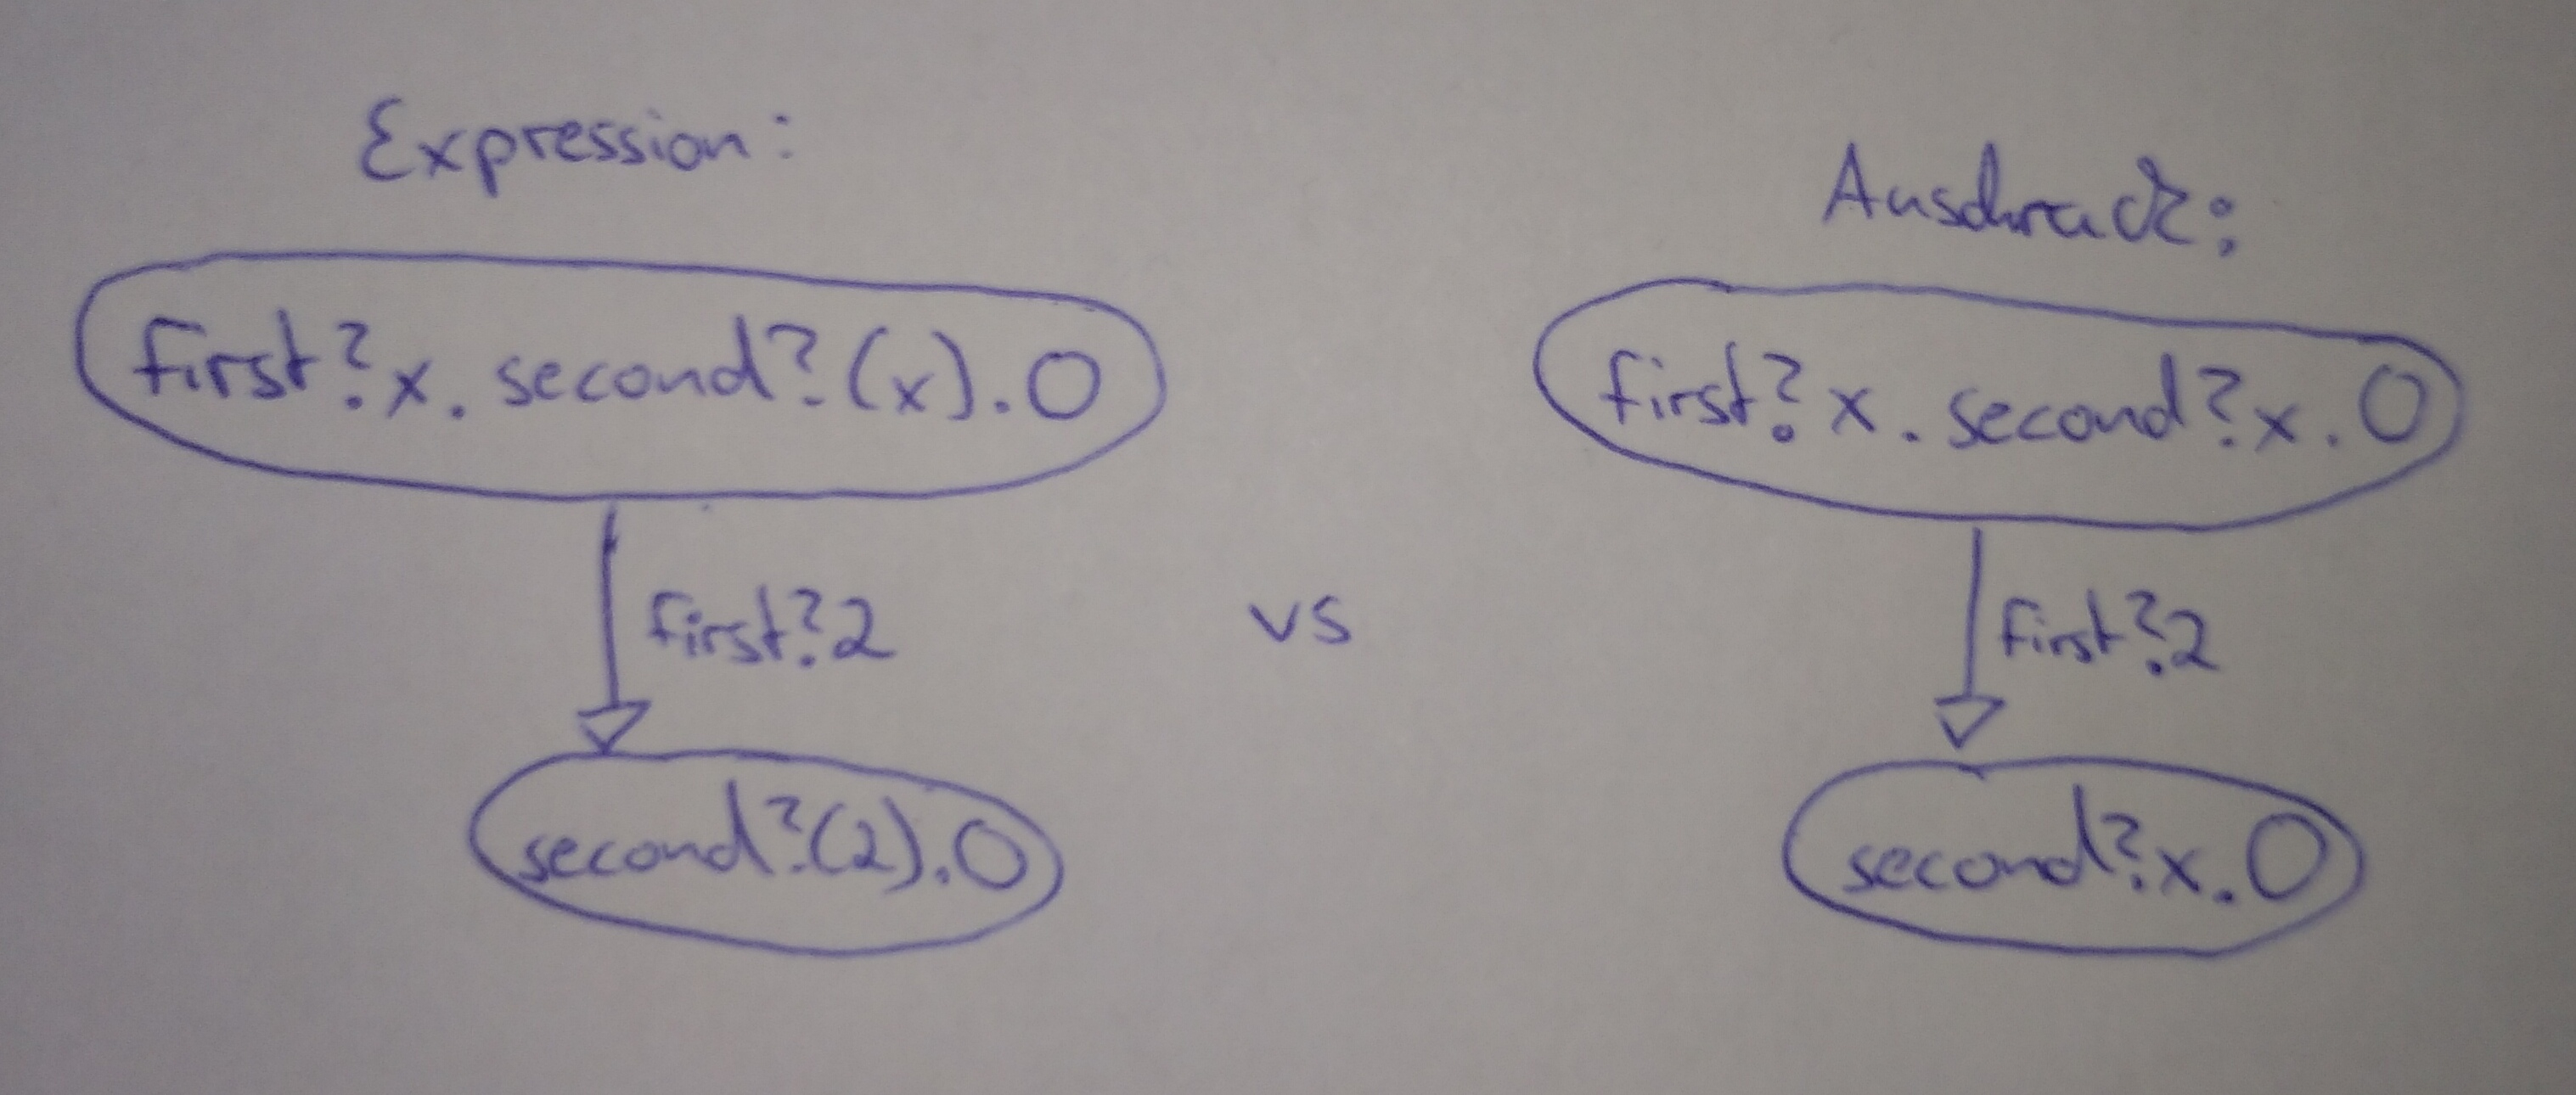
\includegraphics[scale=0.08]{AusdruckVSExpression}
\end{center}


\section{Nützliches und Vorgehensweisen}

\subsubsection*{Relationen im Überblick}
\begin{center}
\begin{tabular}{|l | c c c c c|}
\hline
 & Id(CCS) & $\sim_{iso}$ & $\sim$ & $\sim_{tr}$ & Univ(CCS)\\
 \hline
 Äquivalenzrelation & \checkmark & \checkmark & \checkmark & \checkmark & \checkmark\\
 Kongruenzrelation & \checkmark & \texttimes & \checkmark & \checkmark & \checkmark \\
 erhält Spuren & \checkmark & \checkmark & \checkmark & \checkmark & \texttimes \\
 verklemmungssensitiv & \checkmark & \checkmark & \checkmark & \texttimes & \texttimes \\
 grob genug & \texttimes & \texttimes & \checkmark & \checkmark & \checkmark \\
 \hline
\end{tabular}
\end{center}

\chapter{G: Weil Praxis was für Loser ist}
Ihr wollt Praxis? Hier noch ein paar Definitionen für euch, anstatt darüber zu diskutieren wann es sinnvoll ist sein Programm nebenläufig zu gestalten und welche Vorteile es wirklich bringen könnte. Mit anderen Worten: Warum machen wir das hier eigentlich? Keine Ahnung, hier die Definitionen...

\paragraph{Sequentielle Konsistenz}
Eine mit einem Programm kompatible Ausführung $(J,P,w)$ ist \textit{sequentiell konsistent} wenn es eine totale Ordung $\leq$ auf $J$ gibt, so dass:
\begin{itemize}
 \item $P \subseteq \leq$
 \item für alle $x?v \in J$ gilt:
 \begin{itemize}
  \item $w(x?v) \leq x?v$
  \item es gibt kein $x!v' \not= w(x?v)$ so dass $w(x?v) \leq x!v' \leq x?v$
 \end{itemize}
\end{itemize}

\paragraph{Schwache Konsistenz}
Eine mit einem anderen Programm kompatible Ausführung $(J,P,w)$ ist schwach konsistent, wenn es eine 


\end{document}

